\documentclass{article}
\usepackage{tikz}
\usetikzlibrary{positioning}

\begin{document}

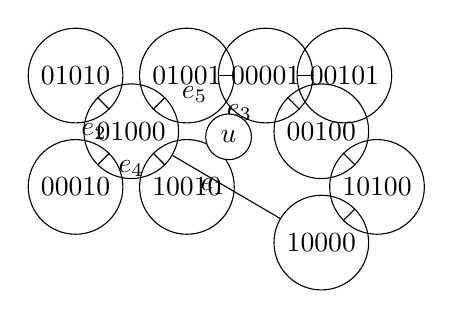
\begin{tikzpicture}[node distance=1cm]
    \tikzstyle{vertex}=[circle,draw,minimum size=0.5cm]

    % Define vertices
    \node[vertex] (v1) at (0,0) {01000};
    \node[vertex] (v2) [above left of=v1] {01010};
    \node[vertex] (v3) [below left of=v1] {00010};
    \node[vertex] (v4) [below right of=v1] {10010};
    \node[vertex] (v5) [above right of=v1] {01001};
    \node[vertex] (v6) [right of=v5] {00001};
    \node[vertex] (v7) [right of=v6] {00101};
    \node[vertex] (v8) [below right of=v6] {00100};
    \node[vertex] (v9) [below right of=v8] {10100};
    \node[vertex] (v10) [below left of=v9] {10000};

    % Draw edges
    \draw (v1) -- (v2);
    \draw (v1) -- (v3);
    \draw (v1) -- (v4);
    \draw (v1) -- (v5);
    \draw (v5) -- (v6);
    \draw (v6) -- (v7);
    \draw (v6) -- (v8);
    \draw (v8) -- (v9);
    \draw (v9) -- (v10);
    \draw (v10) -- (v1);

    % Label edges
    \node at (barycentric cs:v1=1,v2=1,v3=1) {$e_2$};
    \node at (barycentric cs:v1=1,v3=1,v4=1) {$e_4$};
    \node at (barycentric cs:v1=1,v5=1,v6=1) {$e_5$};
    \node at (barycentric cs:v1=1,v6=1,v8=1) {$e_3$};
    \node at (barycentric cs:v1=1,v4=1,v10=1) {$e_1$};

    % Highlight central vertex
    \node[vertex,fill=white] (u) at (barycentric cs:v1=1,v2=1,v3=1,v4=1,v5=1,v6=1,v7=1,v8=1,v9=1,v10=1) {$u$};
\end{tikzpicture}

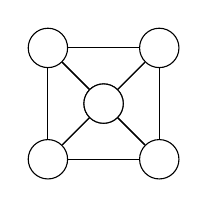
\begin{tikzpicture}[node distance=1cm]
    \tikzstyle{vertex}=[circle,draw,minimum size=0.5cm]

    % Define vertices
    \node[vertex] (v1) at (0,0) {};
    \node[vertex] (v2) [above left of=v1] {};
    \node[vertex] (v3) [above right of=v1] {};
    \node[vertex] (v4) [below right of=v1] {};
    \node[vertex] (v5) [below left of=v1] {};

    % Draw edges
    \draw (v1) -- (v2);
    \draw (v1) -- (v3);
    \draw (v1) -- (v4);
    \draw (v1) -- (v5);
    \draw (v2) -- (v3);
    \draw (v2) -- (v4);
    \draw (v2) -- (v5);
    \draw (v3) -- (v4);
    \draw (v3) -- (v5);
    \draw (v4) -- (v5);

    % Highlight central vertex
    \node[vertex,fill=white] (u) at (barycentric cs:v1=1,v2=1,v3=1,v4=1,v5=1) {};
\end{tikzpicture}

\end{document}